\documentclass[11pt,a4j]{jsarticle}

\usepackage[dvipdfmx]{graphicx}
\usepackage[top=25truemm,bottom=30truemm,left=25truemm,right=25truemm]{geometry}


\usepackage{float,array,booktabs}
\floatstyle{plaintop}

\usepackage{amsmath}
\usepackage{url}

%\restylefloat{figure}
\restylefloat{table}

\begin{document}

\title{AM・FMの通信実験}
\author{hogehoge}
\date{2015年4月26日}
\maketitle

\section{目的}

アナログ通信の中で代表的なAMとFMの通信システムを構成し、各部の動作を確認し、特性を測定し、その原理を理解する。

\section{理論}

\subsection{AM}
\label{sec:am}
AMは振幅を変化させて伝送する。搬送波を$c(t)=A_{c}cos\omega_{c}t$[V]、変調波を$m(t)=A_{m}cos\omega_{t}$[V]とすると出力されるAM信号$u(t)$は

\begin{eqnarray}
u(t)  &=&(A_{c} + A_{m}cos\omega_{m} t ) cos \omega_{c} t  \\
       &=& A_{c} (1+ \frac{A_{m}}{A_{c}} cos \omega_{m} t ) cos \omega_{c} t \label{eq:hentyoudo}\\
       &=& \frac{A_m}{2} cos(\omega_c - \omega_m)t + A_c cos\omega_c t + \frac{A_m}{2} cos(\omega_c + \omega_m) t \,\,\, \mathrm{[V]} \label{eq:sokutaiha}
\end{eqnarray}

となる。このu(t)は以下の図 \ref{ammodel}のような経路をたどって生成される。
\begin{figure}[H]
\begin{center}
	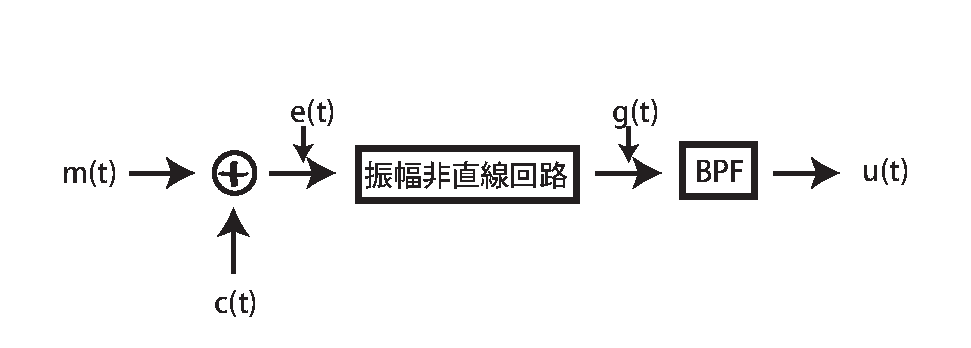
\includegraphics[clip, width=100mm]{amam.eps}
	\caption{AM信号の導出}
	\label{ammodel}
\end{center}
\end{figure}

(\ref{eq:hentyoudo})式の$\frac{A_m}{A_c}$は変調度とよばれ、$K_a$と置かれる。この変調度が1を超えると出力は過変調となる。また(\ref{eq:sokutaiha})式の第1項は下側帯波、第三項は上側帯波とよばれる。第二項は搬送波そのものであり、この波に情報は載っていない。
AM信号では包絡線検波による副長がなされる。図 \ref{fukucho}に包絡線検波の簡単な回路を示す。
\begin{figure}[H]
\begin{center}
	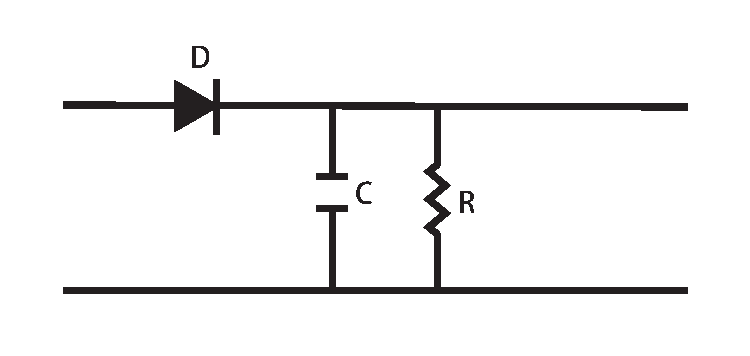
\includegraphics[clip, width=100mm]{am_fukucho.eps}
	\caption{包絡線検波器}
	\label{fig:amdemo}
\end{center}
\end{figure}

\subsection{FM}
FMはAMとは違って、搬送波の振幅は変化させないかわりに、その周波数を変化させることで情報の伝達を行う・搬送波を$m(t)=k_f\times A_mcos\omega_mt\mathrm{[rad / s]}$となる。よって位相が

\begin{eqnarray*}
\phi (t) &=&\int_0^t \omega dt\\
           &=& \omega_c t + \frac{k_fA_m}{\omega_m}sin\omega_mt\mathrm{[rad]}
\end{eqnarray*}

と求められる。これよりFM信号は
\begin{eqnarray*}
u(t) = A_ccos(\omega_c t + \beta sin\omega_m t)
\end{eqnarray*}

\hspace{5mm}

である。なお$\beta = \frac{\displaystyle k_mA_m}{\displaystyle \omega_m}$であり、これを第1種n次ベッセル関数
\begin{align*}
  J_n(\beta) = \frac{1}{\pi}\int_0^{\pi}cos(\, \beta \, sin \xi - n \xi ) \, d \xi
\end{align*}
を用いて展開すると以下のようになる。
\begin{eqnarray}
u(t) = A_c \sum_{n = - \infty}^{\infty} \, J_n(\beta) \, cos(\omega_c + n\omega_m)t \,\,\, \mathrm{[V]}
\label{eq:fm}
\end{eqnarray}

(\ref{eq:fm})式からわかるように$-\infty$から$\infty$までの和であるので理論的には周波数スペクトルは周波数軸上に無限に広がり信号同士の干渉が考えられる。しかし変調指数$\beta$が1よりも十分に大きい場合、カーソンの法則より$2(\beta + 1)\omega_m$に電力の98%が集中するのでエネルギーが高い部分のみを考慮すれば良くなるのである。
FM信号は以下の図\ref{fmgen}の回路により生成される。

\begin{figure}[H]
\begin{center}
	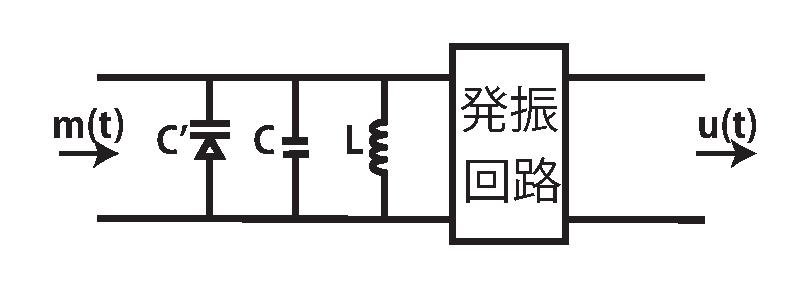
\includegraphics[clip, width=100mm]{fm_gen.eps}
	\caption{FM信号の生成回路}
	\label{fmmo}
\end{center}
\end{figure}

図\ref{fmgen}の一番左の素子はバラクタダイオードといい、電圧によって容量が変化する、可変容量ダイオードである。

またFMの復調には以下の図\ref{fmdemo}の回路が用いられる。
\begin{figure}[H]
\begin{center}
	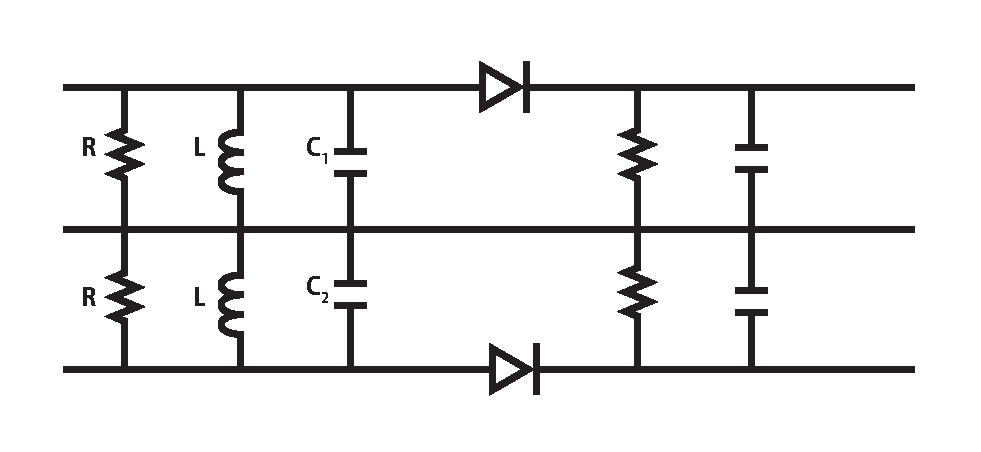
\includegraphics[clip, width=100mm]{fm_demo.eps}
	\caption{FM信号の復調回路}
	\label{fmdemo}
\end{center}
\end{figure}

図\ref{fmdemo}の回路は周波数弁別回路と呼ばれる。またダイオードより左側の部分は上下共振回路と呼ばれ、FMからAMへの変換を行っている。

\section{実験方法}

\subsection{AM変復調実験}

\begin{enumerate}
    \item AM変復調装置、発信機、雑音発声器、オシロスコープ、PCをつないだ。
    \item 発信機の出力を 300Hz、AMPLをひいて-40dBとした。
    \item 変調度が1未満のときの入力信号、変調信号、出力信号を観察し、オシロスコープにつないだPCからモニタに映った様子を保存した。
    \item 雑音発声器を操作して、ノイズ小、ノイズ大における、それぞれの出力内容を同様に観察し、同様に保存した。
    \item 変調度が1の時と、1以上の時における、ノイズなしの出力内容を同様に観察、保存した。
    \item TAによってスペクトルを出力してもらい、発振機が500Hz、800Hz、1200Hz、1500Hzに設定されたそれぞれの場合の変調信号を観察した。
    なお、オシロスコープの横軸は1msecに統一した。
\end{enumerate}

\subsection{FM変復調実験}

\begin{enumerate}
	\item AM変復調装置をFM変調装置とFM復調装置に置き換えて接続した。
	\item 発信機のAMPLを押して、-20dMにした。
	\item 出力が歪まない状態で入力信号、変調信号、出力信号を観察し、オシロスコープにつないだPCからモニタに映った様子を保存した。
	\item AMと同様にノイズ小とノイズ大について、それぞれの出力内容を同様に観察、保存した。
	\item TAによってスペクトルを出力してもらい、発振器が500Hz、800Hz、1200Hz、1500Hzに設定されたそれぞれの場合の変調信号を観察した。
	なお変調信号はPCでのモニタの内容の保存だと信号の揺れを確認できないため、スマートフォンを用いて様子を撮影した。なおオシロスコープの横軸は変調信号の時のみ $50 \mu  \mathrm{s}$、その他の場合は1msとした。
\end{enumerate}





\section{結果}
それぞれの結果を以下の表にまとめた。

%表1
\begin{table}[H]
	\caption{AMノイズなし、変調度1未満}
	\label{tab:am1a} % \ref{ラベル名}で表番号を参照
	\begin{center}
	%表\ref{tab:am1a}: AMノイズなしの変調度1未満
	\begin{tabular}{|c|c|} % l:左寄せ,c:中央揃え r:右寄せ
%	\hline
%	\multicolumn{2}{|c|} {表1: AMノイズなしの変調度1未満}\\
	\hline
	\begin{minipage}{0.5\hsize}
    \centering
    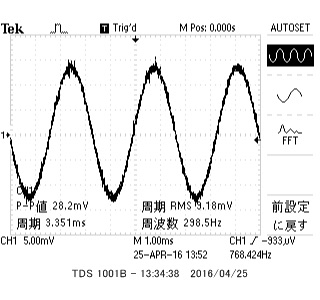
\includegraphics[height=50mm,bb=0 0 320 300]{AM1ain.jpeg} \\
		入力
	\end{minipage} &
	\begin{minipage}{0.5\hsize}
		\begin{center}
			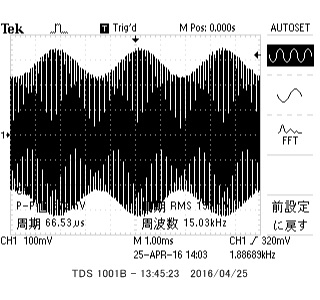
\includegraphics[height=50mm,bb=0 0 320 300]{AM1amo.jpeg} \\
			変調
		\end{center}
	\end{minipage} \\
	\hline
	\begin{minipage}{0.5\hsize}
		\begin{center}
			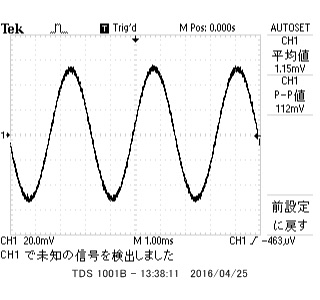
\includegraphics[height=50mm,bb=0 0 320 300]{AM1ademo.jpeg} \\
			復調
		\end{center}
	\end{minipage} &
	\begin{minipage}{0.5\hsize}
		\begin{center}
			変調度$K_a$ \\
			$K_a=\frac{A_m}{A_c}=\frac{350 - 200}{350 + 200}=0.27$
		\end{center}
	\end{minipage} \\   \hline
	\end{tabular}
	\end{center}
\end{table}

%表2
\begin{table}[H]
	\caption{AMノイズ小、変調度1未満}
	\label{tab:am1b} % \ref{ラベル名}で表番号を参照
	\begin{center}
	%表\ref{tab:am1a}: AMノイズなしの変調度1未満
	\begin{tabular}{|c|c|} % l:左寄せ,c:中央揃え r:右寄せ
%	\hline
%	\multicolumn{2}{|c|} {表3: AMノイズ大の変調度1未満}\\
	\hline
	\begin{minipage}{0.5\hsize}
		\begin{center}
			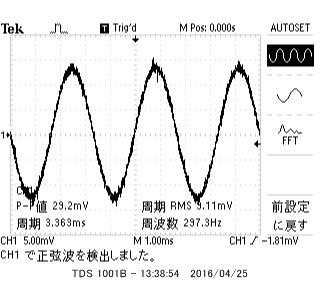
\includegraphics[height=40mm,bb=0 0 320 300]{AM1bin_3.jpeg} \\
			入力
		\end{center}
	\end{minipage} &
	\begin{minipage}{0.5\hsize}
		\begin{center}
			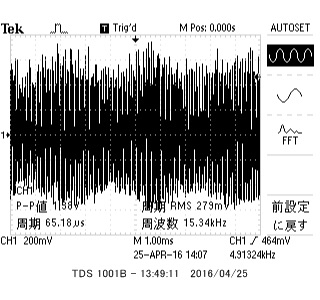
\includegraphics[height=40mm,bb=0 0 320 300]{AM1bmo_3.jpeg} \\
			変調
		\end{center}
	\end{minipage} \\
	\hline
	\begin{minipage}{0.5\hsize}
		\begin{center}
			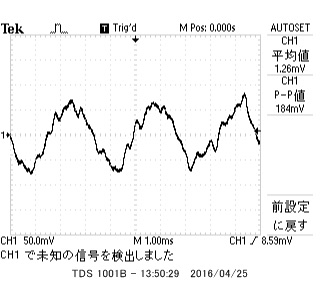
\includegraphics[height=40mm,bb=0 0 320 300]{AM1bdemo_3.jpeg} \\
			復調
		\end{center}
	\end{minipage} &
	\begin{minipage}{0.5\hsize}
		\begin{center}
			変調度$K_a$ \\
			測定不能
		\end{center}
	\end{minipage} \\   \hline
	\end{tabular}
	\end{center}

\end{table}

%表3
\begin{table}[H]
	\caption{AMノイズ大、変調度1未満}
	\label{tab:am1c} % \ref{ラベル名}で表番号を参照
	\begin{center}
	%表\ref{tab:am1a}: AMノイズなしの変調度1未満
	\begin{tabular}{|c|c|} % l:左寄せ,c:中央揃え r:右寄せ
%	\hline
%	\multicolumn{2}{|c|} {表2: AMノイズ小の変調度1未満}\\
	\hline
	\begin{minipage}{0.5\hsize}
		\begin{center}
			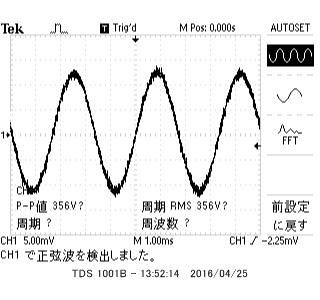
\includegraphics[height=40mm,bb=0 0 320 300]{AM1cin_10.jpeg} \\
			入力
		\end{center}
	\end{minipage} &
	\begin{minipage}{0.5\hsize}
		\begin{center}
			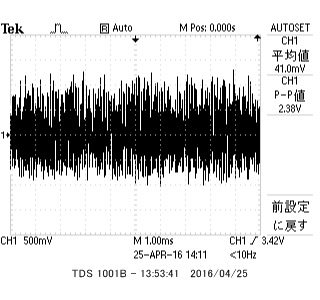
\includegraphics[height=40mm,bb=0 0 320 300]{AM1cmo_10.jpeg} \\
			変調
		\end{center}
	\end{minipage} \\
	\hline
	\begin{minipage}{0.5\hsize}
		\begin{center}
			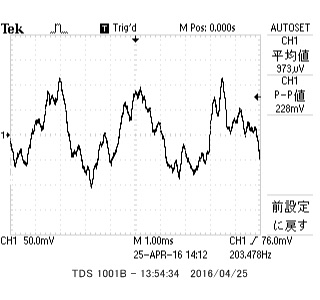
\includegraphics[height=40mm,bb=0 0 320 300]{AM1cdemo_10.jpeg} \\
			復調
		\end{center}
	\end{minipage} &
	\begin{minipage}{0.5\hsize}
		\begin{center}
			変調度$K_a$ \\
			測定不能
		\end{center}
	\end{minipage} \\   \hline
	\end{tabular}
	\end{center}
\end{table}

%表4
\begin{table}[H]
	\caption{AMノイズなし、変調度1}
	\label{tab:am2} % \ref{ラベル名}で表番号を参照
	\begin{center}
	%表\ref{tab:am1a}: AMノイズなしの変調度1未満
	\begin{tabular}{|c|c|} % l:左寄せ,c:中央揃え r:右寄せ
%	\hline
%	\multicolumn{2}{|c|} {表4: AMノイズなしの変調度1}\\
	\hline
	\begin{minipage}{0.5\hsize}
		\begin{center}
			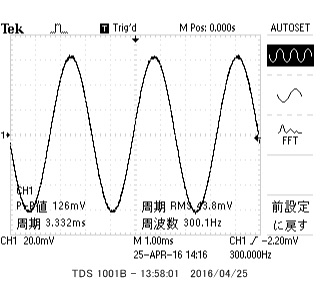
\includegraphics[height=40mm,bb=0 0 320 300]{AM2in.jpeg} \\
			入力
		\end{center}
	\end{minipage} &
	\begin{minipage}{0.5\hsize}
		\begin{center}
			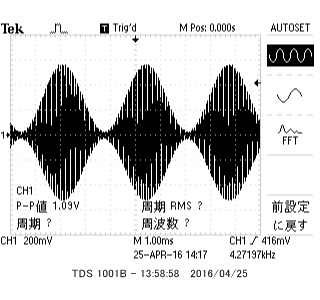
\includegraphics[height=40mm,bb=0 0 320 300]{AM2mo.jpeg} \\
			変調
		\end{center}
	\end{minipage} \\
	\hline
	\begin{minipage}{0.5\hsize}
		\begin{center}
			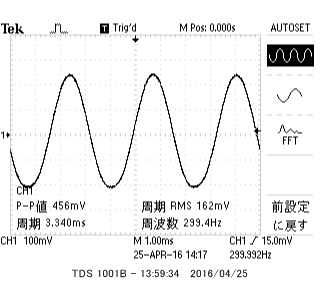
\includegraphics[height=40mm,bb=0 0 320 300]{AM2demo.jpeg} \\
			復調
		\end{center}
	\end{minipage} &
	\begin{minipage}{0.5\hsize}
		\begin{center}
			変調度$K_a$ \\
			$K_a=\frac{A_m}{A_c}=\frac{580 - 10}{580 + 10}=0.97$
		\end{center}
	\end{minipage} \\   \hline
	\end{tabular}
	\end{center}
\end{table}

%表5
\begin{table}[H]
	\caption{AMノイズなし、変調度1以上}
	\label{tab:am3} % \ref{ラベル名}で表番号を参照
	\begin{center}
	%表\ref{tab:am1a}: AMノイズなしの変調度1未満
	\begin{tabular}{|c|c|} % l:左寄せ,c:中央揃え r:右寄せ
%	\hline
%	\multicolumn{2}{|c|} {表5: AMノイズなしの変調度1以上}\\
	\hline
	\begin{minipage}{0.5\hsize}
		\begin{center}
			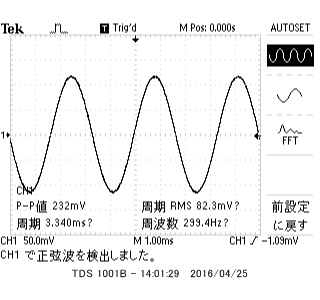
\includegraphics[height=40mm,bb=0 0 320 300]{AM3in.jpeg} \\
			入力
		\end{center}
	\end{minipage} &
	\begin{minipage}{0.5\hsize}
		\begin{center}
			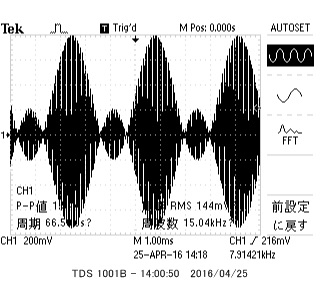
\includegraphics[height=40mm,bb=0 0 320 300]{AM3mo.jpeg} \\
			変調
		\end{center}
	\end{minipage} \\
	\hline
	\begin{minipage}{0.5\hsize}
		\begin{center}
			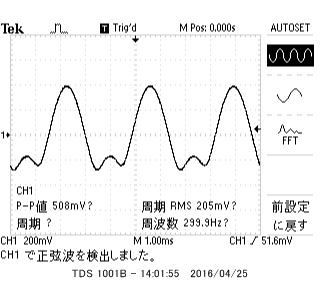
\includegraphics[height=40mm,bb=0 0 320 300]{AM3demo.jpeg} \\
			復調
		\end{center}
	\end{minipage} &
	\begin{minipage}{0.5\hsize}
		\begin{center}
			変調度$K_a$ \\
			$K_a=\frac{A_m}{A_c}=\frac{800 - (-200)}{800 + (-200)}=1.67$
		\end{center}
	\end{minipage} \\   \hline
	\end{tabular}
	\end{center}
\end{table}

%表6
\begin{table}[H]
	\caption{FMノイズなし、歪みなし}
	\label{tab:fm1a} % \ref{ラベル名}で表番号を参照
	\begin{center}
	%表\ref{tab:am1a}: AMノイズなしの変調度1未満
	\begin{tabular}{|c|c|} % l:左寄せ,c:中央揃え r:右寄せ
%	\hline
%	\multicolumn{2}{|c|} {表6: FMノイズなし歪みなし}\\
	\hline
	\begin{minipage}{0.5\hsize}
		%\begin{center}
		\centering

			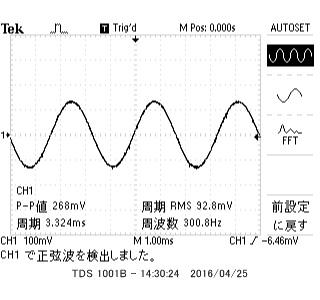
\includegraphics[height=40mm,bb=0 0 320 300]{FM1ain.jpeg} \\
			入力
		%\end{center}
	\end{minipage} &
	\begin{minipage}{0.5\hsize}
		%\begin{center}
		\centering
			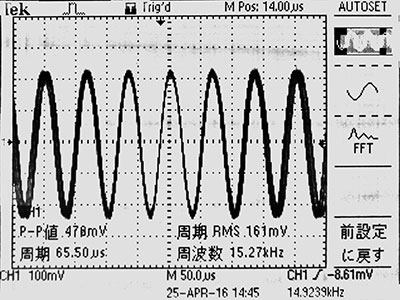
\includegraphics[height=40mm,bb=0 0 400 300]{FM1amo.jpeg} \\
			変調
		%\end{center}
	\end{minipage} \\
	\hline
	\begin{minipage}{0.5\hsize}
		%\begin{center}
		\centering
			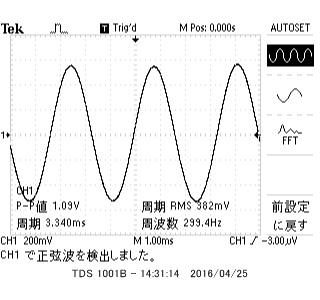
\includegraphics[height=40mm,bb=0 0 320 300]{FM1ademo.jpeg} \\
			復調
		%\end{center}
	\end{minipage} &
	 \\   \hline
	\end{tabular}
	\end{center}
\end{table}

%表7
\begin{table}[H]
	\caption{FMノイズなし、歪みあり}
	\label{tab:fm1b} % \ref{ラベル名}で表番号を参照
	\begin{center}
	%表\ref{tab:am1a}: AMノイズなしの変調度1未満
	\begin{tabular}{|c|c|} % l:左寄せ,c:中央揃え r:右寄せ
%	\hline
%	\multicolumn{2}{|c|} {表7: FMノイズなし歪みあり}\\
	\hline
	\begin{minipage}{0.5\hsize}
		%\begin{center}
		\centering

			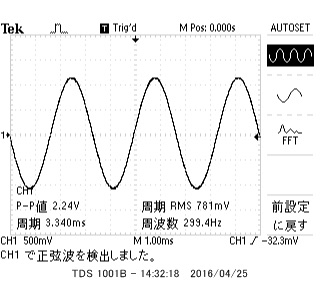
\includegraphics[height=40mm,bb=0 0 320 300]{FM1bin.jpeg} \\
			入力
		%\end{center}
	\end{minipage} &
	\begin{minipage}{0.5\hsize}
		%\begin{center}
		\centering
			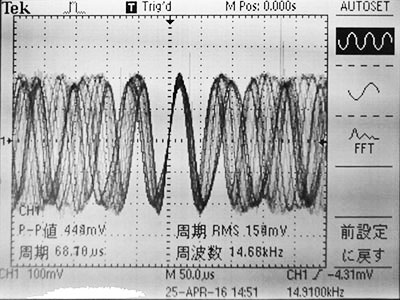
\includegraphics[height=40mm,bb=0 0 400 300]{FM1bmo.jpeg} \\
			変調
		%\end{center}
	\end{minipage} \\
	\hline
	\begin{minipage}{0.5\hsize}
		%\begin{center}
		\centering
			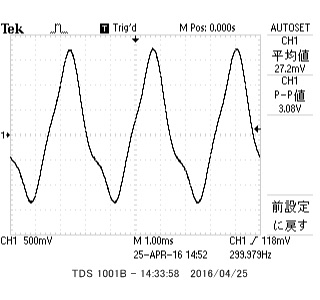
\includegraphics[height=40mm,bb=0 0 320 300]{FM1bdemo.jpeg} \\
			復調
		%\end{center}
	\end{minipage} &
	 \\   \hline
	\end{tabular}
	\end{center}
\end{table}


%表8
\begin{table}[H]
	\caption{FMノイズ小、歪みなし}
	\label{tab:fm2c} % \ref{ラベル名}で表番号を参照
	\begin{center}
	%表\ref{tab:am1a}: AMノイズなしの変調度1未満
	\begin{tabular}{|c|c|} % l:左寄せ,c:中央揃え r:右寄せ
%	\hline
%	\multicolumn{2}{|c|} {表8: FMノイズ小歪みなし}\\
	\hline
	\begin{minipage}{0.5\hsize}
		%\begin{center}
		\centering

			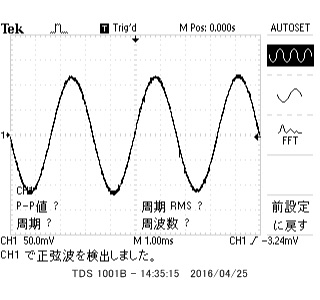
\includegraphics[height=40mm,bb=0 0 320 300]{FM2cin_3.jpeg} \\
			入力
		%\end{center}
	\end{minipage} &
	\begin{minipage}{0.5\hsize}
		%\begin{center}
		\centering
			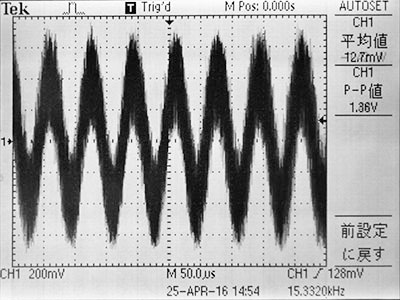
\includegraphics[height=40mm,bb=0 0 400 300]{FM2cmo_3.jpeg} \\
			変調
		%\end{center}
	\end{minipage} \\
	\hline
	\begin{minipage}{0.5\hsize}
		%\begin{center}
		\centering
			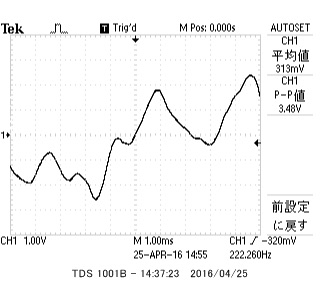
\includegraphics[height=40mm,bb=0 0 320 300]{FM2cdemo_3.jpeg} \\
			復調
		%\end{center}
	\end{minipage} &
	 \\   \hline
	\end{tabular}
	\end{center}
\end{table}


%表9
\begin{table}[H]
	\caption{FMノイズ大、歪みなし}
	\label{tab:fm2d} % \ref{ラベル名}で表番号を参照
	\begin{center}
	%表\ref{tab:am1a}: AMノイズなしの変調度1未満
	\begin{tabular}{|c|c|} % l:左寄せ,c:中央揃え r:右寄せ
%	\hline
%	\multicolumn{2}{|c|} {表9: FMノイズ大歪みなし}\\
	\hline
	\begin{minipage}{0.5\hsize}
		%\begin{center}
		\centering

			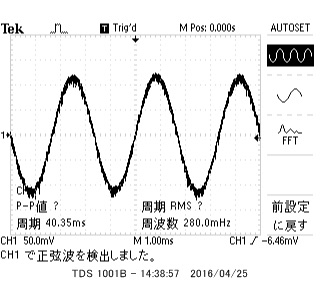
\includegraphics[height=40mm,bb=0 0 320 300]{FM2din_10.jpeg} \\
			入力
		%\end{center}
	\end{minipage} &
	\begin{minipage}{0.5\hsize}
		%\begin{center}
		\centering
			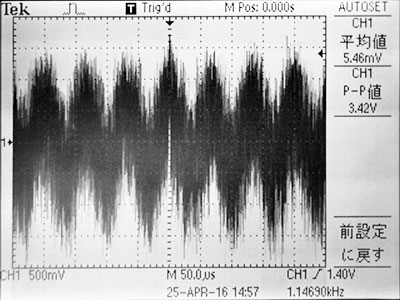
\includegraphics[height=40mm,bb=0 0 400 300]{FM2dmo_10.jpeg} \\
			変調
		%\end{center}
	\end{minipage} \\
	\hline
	\begin{minipage}{0.5\hsize}
		%\begin{center}
		\centering
			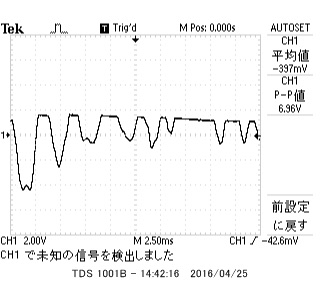
\includegraphics[height=40mm,bb=0 0 320 300]{FM2ddemo_10.jpeg} \\
			復調
		%\end{center}
	\end{minipage} &
	 \\   \hline
	\end{tabular}
	\end{center}
\end{table}


%表10
\begin{table}[H]
	\caption{AMスペクトル}
	\label{tab:ams} % \ref{ラベル名}で表番号を参照
	\begin{center}
	%表\ref{tab:am1a}: AMノイズなしの変調度1未満
	\begin{tabular}{|c|c|} % l:左寄せ,c:中央揃え r:右寄せ
%	\hline
%	\multicolumn{2}{|c|} {表10: AMスペクトル}\\
	\hline
	\begin{minipage}{0.5\hsize}
		%\begin{center}
		\centering
		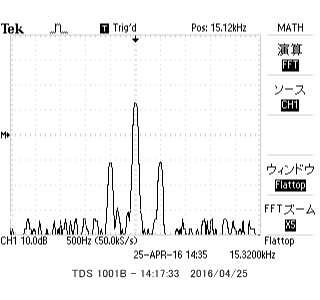
\includegraphics[height=40mm,bb=0 0 320 300]{AM500Hz.jpeg} \\
		AMスペクトル 500Hz
		%\end{center}
	\end{minipage} &
	\begin{minipage}{0.5\hsize}
		%\begin{center}
		\centering
		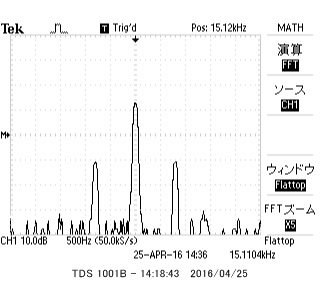
\includegraphics[height=40mm,bb=0 0 320 300]{AM800Hz.jpeg} \\
		AMスペクトル 800Hz
		%\end{center}
	\end{minipage} \\
	\hline
	\begin{minipage}{0.5\hsize}
		%\begin{center}
		\centering
		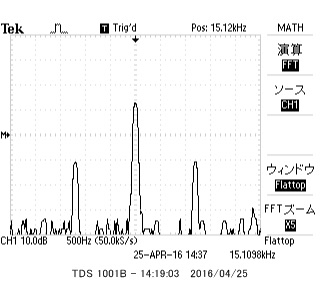
\includegraphics[height=40mm,bb=0 0 320 300]{AM1200Hz.jpeg} \\
		AMスペクトル 1200Hz
		%\end{center}
	\end{minipage} &
	\begin{minipage}{0.5\hsize}
		%\begin{center}
		\centering
		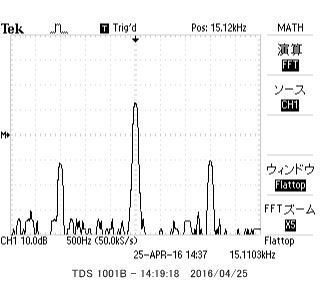
\includegraphics[height=40mm,bb=0 0 320 300]{AM1500Hz.jpeg} \\
		AMスペクトル 1500Hz
		%\end{center}
	\end{minipage}	 \\   \hline
	\end{tabular}
	\end{center}
\end{table}


%表11
\begin{table}[H]
	\caption{FMスペクトル}
	\label{tab:fms} % \ref{ラベル名}で表番号を参照
	\begin{center}
	%表\ref{tab:am1a}: AMノイズなしの変調度1未満
	\begin{tabular}{|c|c|} % l:左寄せ,c:中央揃え r:右寄せ
%	\hline
%	\multicolumn{2}{|c|} {表11: FMスペクトル}\\
	\hline
	\begin{minipage}{0.5\hsize}
		%\begin{center}
		\centering
		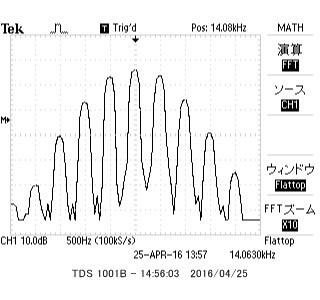
\includegraphics[height=40mm,bb=0 0 320 300]{FM1500Hz.jpg} \\
		\vspace{-4mm}
		FMスペクトル 500Hz
		%\end{center}
	\end{minipage} &
	\begin{minipage}{0.5\hsize}
		%\begin{center}
		\centering
		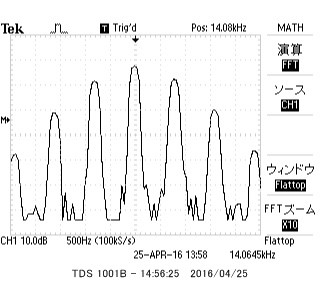
\includegraphics[height=40mm,bb=0 0 320 300]{FM1200Hz.jpg} \\
		\vspace{-4mm}
		FMスペクトル 800Hz
		%\end{center}
	\end{minipage} \\
	\hline
	\begin{minipage}{0.5\hsize}
		%\begin{center}
		\centering
		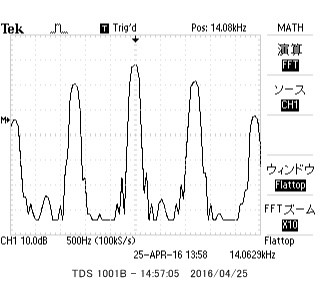
\includegraphics[height=40mm,bb=0 0 320 300]{FM800Hz.jpg} \\
		\vspace{-4mm}
		FMスペクトル 1200Hz
		%\end{center}
	\end{minipage} &
	\begin{minipage}{0.5\hsize}
		%\begin{center}
		\centering
		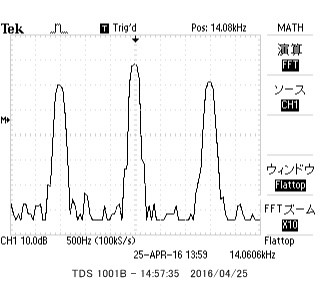
\includegraphics[height=40mm,bb=0 0 320 300]{FM500Hz.jpg} \\
		\vspace{-4mm}
		FMスペクトル 1500Hz
		%\end{center}
	\end{minipage}	 \\   \hline
	\end{tabular}
	\end{center}
\end{table}

\section{考察}

\subsection{周波数スペクトクラムの理論的導出}
\ref{sec:am}の(\ref{eq:sokutaiha})式より、AM信号は3つの余弦波によって構成される。
そのため振幅スペクトルの概形も3つの値が大きくなり、両脇の二つの振幅の値は等しくなることは式からわかる。
これらは表\ref{tab:ams}の結果をみても一致している。

そして、入力波の周波数($\omega_m$)を大きくしていくと実験結果も示す通り、上側帯波と下側帯波が離れていく。

FMについては、式\ref{eq:fm}を考える。
この式を展開すると、
\begin{align}
  u(t) = A_c \,\{\cdots + J_{-1}(\beta)cos(\omega_c - \omega_m)t + J_0(\beta)cos(\omega_c - \omega_m)t + J_1(\beta)cos(\omega_c - \omega_m)t + \cdots \, \}
\end{align}

となる。ベッセル関数の$J_n(\beta)$は係数なので、スペクトルには影響しない。信号の周波数スペクトルはAM信号のように中心$\omega_c$から$\omega_m$の整数倍離れたところに振幅を持つ。
つまり、各スペクトルは等間隔である。ただ、ベッセル関数は減衰関数なので中心周波数から離れるほど振幅は小さくなる。
また、AMと同様に入力の周波数をあげるとその間隔は広くなる。これは実験結果をみても明らかである。

\subsection{過変調での出力結果の歪み}
過変調は変調波の振幅が搬送波の振幅を超えている状態である。
変調度が1以下の場合では、包絡線は波の中心を超えることがないので検波の際には正しい出力波を得られる。
しかしながら、過変長の場合は、包絡線の波の中心を超えた部分が検波時に切り取られてしまうので入力と異なった形の波形が出力されるため歪みが発生する。
一方で、FMの場合はフィルタの周波数特性により、ある一定の範囲では周波数と電圧の線形関係が成り立っている。
ただし、その範囲を超えた周波数はその関係が成り立たない。
過変調の場合はその状態にあるので、出力波形が複雑な歪みを作る。
したがってAMとFMの場合で歪み方が異なるのは、歪みを発生させる原因か異なっており、゙その影響を受ける部分も異なるためであると考えられる。

\subsection{雑音が与える影響}
AM変調に雑音を混ぜると、スピーカーから徐々に「ザー」という音が聞こえてきて、最大にしたとき元の音は聞こえない程となった。
FM変調ではすこしずつ雑音が聞こえてきて、ある程度まで雑音を大きくしたら元の音を含め雑音は聞こえなくなった。
AMでは雑音の波を入力に加えることで表\ref{tab:am1b},表\ref{tab:am1c}のように出力の波形が乱れてしまうため雑音が聞こえるようになる。
雑音が大きくなるにつれ入力波形への影響は大きくなるので雑音が徐々に大きくなる。
FMでは搬送波の周波数に情報を乗せるため振幅方向の雑音はAMほどの影響を受けない。
音が聞こえなくなったのは雑音による入力信号のぶれが一定以上の大きさになると、どの周波数に情報がのっているのかがわからなくなり、復調できなくなるものと考えられる。
よってFM変調のほうが雑音に強いと考えられる。

\subsection{搬送波に正弦波を利用する理由}
フーリエ級数展開とは周期関数をさまざまな正弦波の重ね合わせとして表すものである。
つまり、異なる周波数の正弦波を混合した電気信号はフーリエ級数展開によって容易に各周波数に分離できる。
そのため、搬送波には正弦波を利用すると考えられる。


\subsection{AM検波}
図\ref{fig:amdemo}がAMの検波を行う回路である。左半分のダイオードで半端清流を行って、入力信号の片方を取り出して、それを右半分のLPFに送ることで、定周波数成分のみを取り出して包絡線を得ている。

\subsection{FM$\rightarrow$AMの変換}
図\ref{fmdemo}を見てみると、回路は周波数弁別回路と包絡線検波で用いた積分回路の組み合わせとなっている。
AM→FM 変換部分では2つの共振回路によってバンドパスフィルタを作っている。その共振周波数はそれぞれ、

$\frac{1}{\sqrt{L_1C}} \, , \, \frac{1}{\sqrt{L_2C}}$

となっている。この周波数の時に出力電圧が最大となる。回路の入出力特性は、

$\frac{1}{\sqrt{L_1C}} < \omega < \frac{1}{\sqrt{L_2C}}$

において、周波数と電圧が比例関係となる。

検波される波の周波数の変化が出力電圧の変化となるので、AMでの変調波の波形のように横軸時間、縦軸電圧の波形が出力される。
つまりFM→AM変換がなされる。

\subsection{AM、FM、テレビと搬送波の周波数が高くなる理由}
搬送波周波数を高くすると、周波数帯域を広く確保することが容易となる。
そのため、より品質のいいデータを送るためには高周波数を利用することが必要になる。
テレビがラジオと比較して、品質が良くデータ量が大きのはもちろんのことだが、FMとAMラジオを比較しても、FMの方が高品質である。
このように品質のいいデータを送るために高い周波数を利用していると考えられる。

\subsection{通信防災室の感想}
いろいろな生活に関連する電波(テレビや、携帯など)の波を見て、見えていなくとも、ありとあらゆる種類の電波が飛び交っているんだなと思った。




\section{ラジオ}

%表12 radio
\begin{table}[H]
	\caption{受信報告書}
	\label{tab:radio}
	\begin{center}
	\begin{tabular}{|c|c|c|c|c|c|c|} % l:左寄せ,c:中央揃え r:右寄せ
	\hline
	周波数 & 受信時間 & 番組内容 & S & I & N & O \\
	\hline
	81.3MHz & 15:20 & 音楽番組 & 3 & 5 & 2 & 2 \\
	\hline
	80.0MHz & 15:22 & トーク番組(FM横浜) & 5 & 5 & 4 & 4 \\
	\hline
	77.1MHz & 15:24 & 産業の話の講義(放送大学) & 4 & 5 & 4 & 4 \\
	\hline
	954kHz & 15:25 & 不明 & 5 & 5 & 1 & 1 \\
	\hline
	メモし忘れ & 15:28 & 航空無線 & 2 & 5 & 3 & 4 \\
	\hline
	15.415MHz & 15:31 & 外国語のラジオ & 3 & 5 & 2 & 2 \\
	\hline
	13.650MHz & 15:32 & 韓国の音楽番組 & 3 & 5 & 2 & 3 \\
	\hline
	9.730MHz & 15:35 & 北朝鮮のラジオ & 1 & 5 & 1 & 1 \\
	\hline
	9.445MHz & 15:35 & ?(北朝鮮のラジオとのこと) & 5 & 5 & 1 & 1 \\
	\hline
	\end{tabular}
	\end{center}
\end{table}


\begin{thebibliography}{99}
\bibitem{keio} 慶應義塾大学理工学部電気系共通実験室,2004 年度情報工学実験第 1 実験指導
書「AM と FM の通信実験」.
\bibitem{radio1} Radio GXK, 「H14年08月期 A-15  Code:[HF0105] : 各種通信方式の復調における得失比較」, \url{http://www.gxk.jp/elec/musen/1ama/H14/html/H1408A15_.html} ,参照日(2016/04/30).
\bibitem{radio2} Radio GXK, 「H21年04月期 A-13  Code:[HE0305] : 振幅変調波形のピークと谷から変調度を求める」, \url{http://www.gxk.jp/elec/musen/1ama/H21/html/H2104A13_.html} ,参照日(2016/04/30).
\end{thebibliography}


\end{document}
